\begin{multicols}{3}[\section{C-Netz}]

\rhead{Daniel Keilmann, Lucas Heuser}
\lfoot{18.05.2016}

\newrefsegment

\begin{tabular}{p{2,1 cm}p{2.7 cm}}
\textbf{Steckbrief}& \\
\end{tabular}
\rowcolors{1}{\topicolor!20}{}
\begin{tabular}{p{2,1 cm}p{2.7 cm}}
      Einsatz seit & 01.05.1985\\
	  Eingestellt am & 31.12.2000\\
	  Auslastung & 850.000 Teilnehmer\\
      Frequenz"-bereich  & Unterband: \SI{451,30}-\SI{455,74}{\mega\hertz}
						   Oberband: \SI{461,30}-\SI{465,74}{\mega\hertz} \\
      Verbreitung & DE, PT und ZA\\
      Modulation & Phasenmodulation (14F3), \newline
	               Frequenzmodulation (binär)\\
      Sendeleistung & Feststation: \newline max. \SI{25} Watt \newline
				      Teilnehmer: \newline max. \SI{15} Watt\\
\end{tabular}
\par
%Source http://www.fh-bingen.de/fileadmin/user_upload/Lehrende/Kilsch_Dieter/internet/projekte/TedoSchStiUnits.pdf -> Seite 9 findet ihr alle verwendbaren Einheiten, wie:
%\SI{Zahl}{\mega\hertz} oder \SI{Zahl}{\mili\metre}
%Ich weiß ehrlich gesagt nicht welche Einheiten ihr im Text genau braucht, aber in dem Dokument und mit obigen Beispiel sollte es umsetzbar ein.
\subsection*{Überblick}
\begin{wrapfigure}{r}{0.4\linewidth}
  \vspace{-20pt}
  \begin{center}
  	\hspace{-20pt}
    
\includegraphics[width=0.7\linewidth]{Kapitel/C-Netz/Grafiken/C-Netz_Logo.png}
  \end{center}
  \vspace{-15pt}
\end{wrapfigure}
Das C-Netz der \textit{DeTeMobil} (ehemals: \textit{Deutsche Bundespost TELEKOM}) war seit Mitte 1984 verfügbar und startete offiziell im September 1985. Ende 2000 wurde der Betrieb eingestellt. \enquote{Anders als beim B-Netz betrieben die Nachbarländer Netze mit einem anderen technischen Standard, sodass die deutsche Form des C-Netzes nur noch in Portugal und Südafrika genutzt wurde.}~\cite{c-netz.1}\\
Zu dem Thema C-Netz wird im weiteren Verlauf auf die folgenden Aspekte eingegangen:
\begin{itemize}
	\item Technische Erläuterung
	\item Vergleich zum A- und B-Netz 
	\item Einsatz		
	\item Anbieter und Gremien
	\item Historische Entwicklung
	\item Ausblick
\end{itemize}



\subsection*{Technische Erläuterung}
Eine flächendeckende Versorgung wurde in Großzellen (Radius von 15-20 km) und Kleinzellen (2–3 km) in den Ballungsräumen realisiert. In den Anfangsjahren bestand das C-Netz aus zwei Funkvermittlungsstellen und 175 Funkzonen, beziehungsweise Funkfeststationen. Das C-Netz konnte (im Endausbau) 850.000 Teilnehmer aufnehmen. Aktivierte Funkverbindungen wurden beim Wechsel der Funkzelle automatisch weitergereicht (Handover, siehe Abb. \ref{fig:c-netz.handover}). 
\begin{Figure}
\includegraphics[width=\linewidth]{Kapitel/C-Netz/Grafiken/handover.png}
\captionof{figure}{Schematische Darstellung eines Handovers beim Funkzellenwechsel}
\label{fig:c-netz.handover}
\end{Figure}
Der C-Netz-Teilnehmer hatte im gesamten Versorgungsbereich eine einheitliche Zugangskennzahl (0161) und Funkrufnummer, über die er erreichbar war. Mängel des C-Netzes waren die begrenzte Teilnehmeranzahl, die vergleichsweise geringe Sprachqualität und das erhöhte Abhörrisiko. Durch die Sprachverschleierung sollte das Abhörrisiko verringert werden, führte aber lediglich eine Invertierung des Sprachbandes aus. Dies konnte mit geringen technischen Mitteln umgangen werden. Bei schlechten Verbindungen konnte der Benutzer diese ausschalten und damit die Verständlichkeit erhöhen.
Das C-Netz-System unterstützte als erstes System die Trennung von Teilnehmeridentität und Endgerät. Die Teilnehmeridentität, beziehungsweise die Zugangsberechtigung waren auf einer Magnetkarte kodiert. Das heißt, durch das Einschieben dieser Karte wurde ein beliebiges Mobiltelefon einem Nutzer zugeordnet. Im Jahre 1988 wurde der Magnetstreifen durch die TeleKarte mit integriertem Mikrokontroller ersetzt. Dies war der Vorläufer der heute verwendeten \textbf{SIM}-Karte (\textbf{S}ubscriber \textbf{I}dentity \textbf{M}odule).
\begin{Figure}
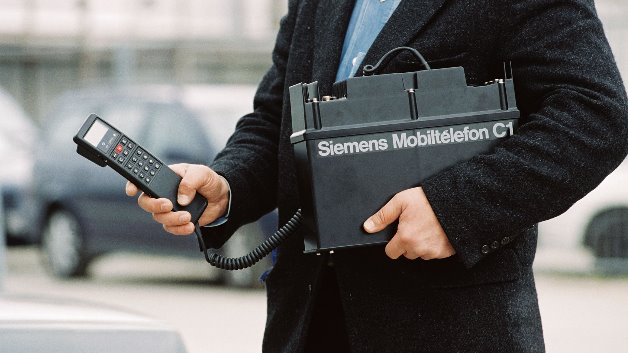
\includegraphics[width=\linewidth]{Kapitel/C-Netz/Grafiken/MobiltelefonC1.jpg}
\captionof{figure}{Mobiltelefon~\cite{c-netz.2}}
\label{fig:c-netz.mobiltelefonEins}
\end{Figure}
Für die damalige Zeit ungewöhnlich waren auch die funktional reich bestückten Hörer, die alle Bedienelemente, LC-Display und LEDs besaßen. 
Das Tastenset war gemäß der \textit{\textbf{CCITT}}-Empfehlungen (\textit{\textbf{C}omité \textbf{C}onsultatif \textbf{I}nternational \textbf{T}éléphonique et \textbf{T}élégraphique}) aufgebaut und die weitere Mensch-Maschine-Schnittstelle war nach einer \textit{\textbf{FTZ}}-Richtlinie (\textit{\textbf{F}ernmelde\textbf{t}echnisches \textbf{Z}entralamt}) für alle Hersteller geregelt, so dass der Nutzer keine gerätespezifischen Umstellungsschwierigkeiten hatte, sondern grundsätzlich Zustände wie „eingebucht“, „verbunden“ oder „Sprachverschleierung eingeschaltet“ in bekannter Form angezeigt bekam.

Die Übertragung von Signalisierungsdaten, wurde realisiert durch die Unterteilen des Audiosignals in jeweils 12,5 ms lange Audioblöcke und deren 10 prozentige, zeitliche Kompression, um in die so entstandenen 1,25 ms langen Lücken 4-Bit-Datentelegramme einzufügen.



\subsubsection*{Vergleich zum A- und B-Netz}
„Das C-Netz bot im Vergleich zu den dahin bekannten analogen Mobilnetzen eine Handover-Funktion, die nicht nach der Feldstärke gesteuert wurde, sondern von der relativen Entfernung zur Basisstation. Damit waren die Handover auch schon unter besten Funkbedingungen möglich, was bei der Netzplanung und der Verdichtung der Frequenzwiederholung ein sehr nützliches Merkmal war. Auch wurde damit die Gleichkanalstörwahrscheinlichkeit deutlich reduziert. Um die relative Entfernungsmessung unterstützen zu können, war jedoch zusätzlicher technischer Aufwand nötig, nämlich eine zeitliche Synchronisation aller Basisstationen zueinander.“~\cite{c-netz.3}  Für das Realisieren auf Bundesebene beziehungsweise für das Netz an sich, besaß jede Basisstation spezifische Sender und Empfänger für Synchronisationssignale.
Gegenüber dem A-Netz und B-Netz gab es im C-Netz viele „bahnbrechende“ Neuerungen, die heute längst selbstverständlich sind. Beispiele hierfür sind:
\begin{itemize}
	\item Gemeinsame Vorwahl (0161-) für alle Mobil-Teilnehmer. Man braucht im Gegensatz zum A- und B-Netz nicht mehr zu wissen, wo sich der Teilnehmer aufhält.
	\item Unterbrechungsfreier Wechsel von einer Funkstation zur nächsten (Handover)
	\item Verschleierung des (analogen) Funksignals erschwert unberechtigtes Abhören
	\item Neben fest eingebauten Geräten auch herausnehmbare oder sogar tragbare Geräte möglich
	\item Bis zu 850.000 Teilnehmer (A-Netz 10.500, B-Netz 27.000)
	\item Seit Ende 1990 Anrufbeantworter und Ruf-umleitung als Netzmerkmal (bis dahin nur als Hardware-Zubehör)~\cite{c-netz.3}
\end{itemize}



\subsection*{Einsatz}
Das C-Netz (Funktelefonnetz-C) war ein analoges, zellulares Mobilfunknetz der deutschen \textit{DeTeMobil}. Es war die dritte und gleichzeitig auch letzte analoge Generation des Mobilfunks, die als System nur in Deutschland, Portugal und Südafrika eingesetzt wurde. Die sehr gute Netzabdeckung von fast 100 Prozent machte das C-Netz zu einer sehr komfortablen Alternative zu den bisherigen Netzen. Das C-Netz wurde primär für telefonische Kommunikationsanwendungen (Autotelefonnetz) mit Zugang zum Telefonnetz und \textbf{ISDN} (\textbf{I}ntegrated \textbf{S}ervices \textbf{D}igital \textbf{N}etwork) konzipiert. Das C-Netz wurde vorwiegend für Autotelefone, Küstenschiffe und Eisenbahntelefone benutzt~\cite{c-netz.1}.
Am 31. Dezember 1988 gab es bundesweit bereits 98.762 und im Land Berlin 2.076 C-Netz-Teilnehmer~\cite{c-netz.3}.
Der Betrieb des C-Netzes wurde am 31. Dezember 2000 eingestellt~\cite{c-netz.6}. Das praktisch unmögliche Roaming in Netze der Nachbarländer war hierfür der Hauptgrund und ebenso der Grundstein für die Entwicklung der nächsten Netztechnologie, die erstmals mit dem D-Netz ab 1992 zum Einsatz kam.




\subsection*{Anbieter und Gremien}
Das C-Netz wurde in Deutschland ausschließlich von der \textit{Telekom Deutschland GmbH} (ehemals: \textit{Deutsche Bundespost Telekom} und \textit{DeTeMobil}) zur Verfügung gestellt, die dies im Auftrag des Deutschen Staates umsetzte. Zu den Telefonherstellern gehören unter anderem \textit{AEG}, \textit{Bosch}, \textit{Nokia}, \textit{Siemens} und noch viele Weitere~\cite{c-netz.5}.

Das C-Netz wurde im Jahre 1984 (offiziell 1985) in Deutschland eingeführt und ersetzte die umständliche Handhabung des B- beziehungsweise B2-Netzes (Fräulein vom Amt/manueller Verbindungsaufbau). Es war auf Deutschland, Portugal und Südafrika beschränkt, hatte aber mit einer Netzabdeckung von fast 100 Prozent einen höheren Verbreitungsgrad als das digitale D-Netz bei der Einführung (1991). Dadurch wurde das C-Netz bei Autotelefonen noch bis Mitte der 90er Jahre als erste Wahl eingesetzt, weil es besonders in den ländlichen Gebieten eine bessere Erreichbarkeit hatte als das C-Netz. 


\end{multicols}
\newpage
\section*{Historische Entwicklung}
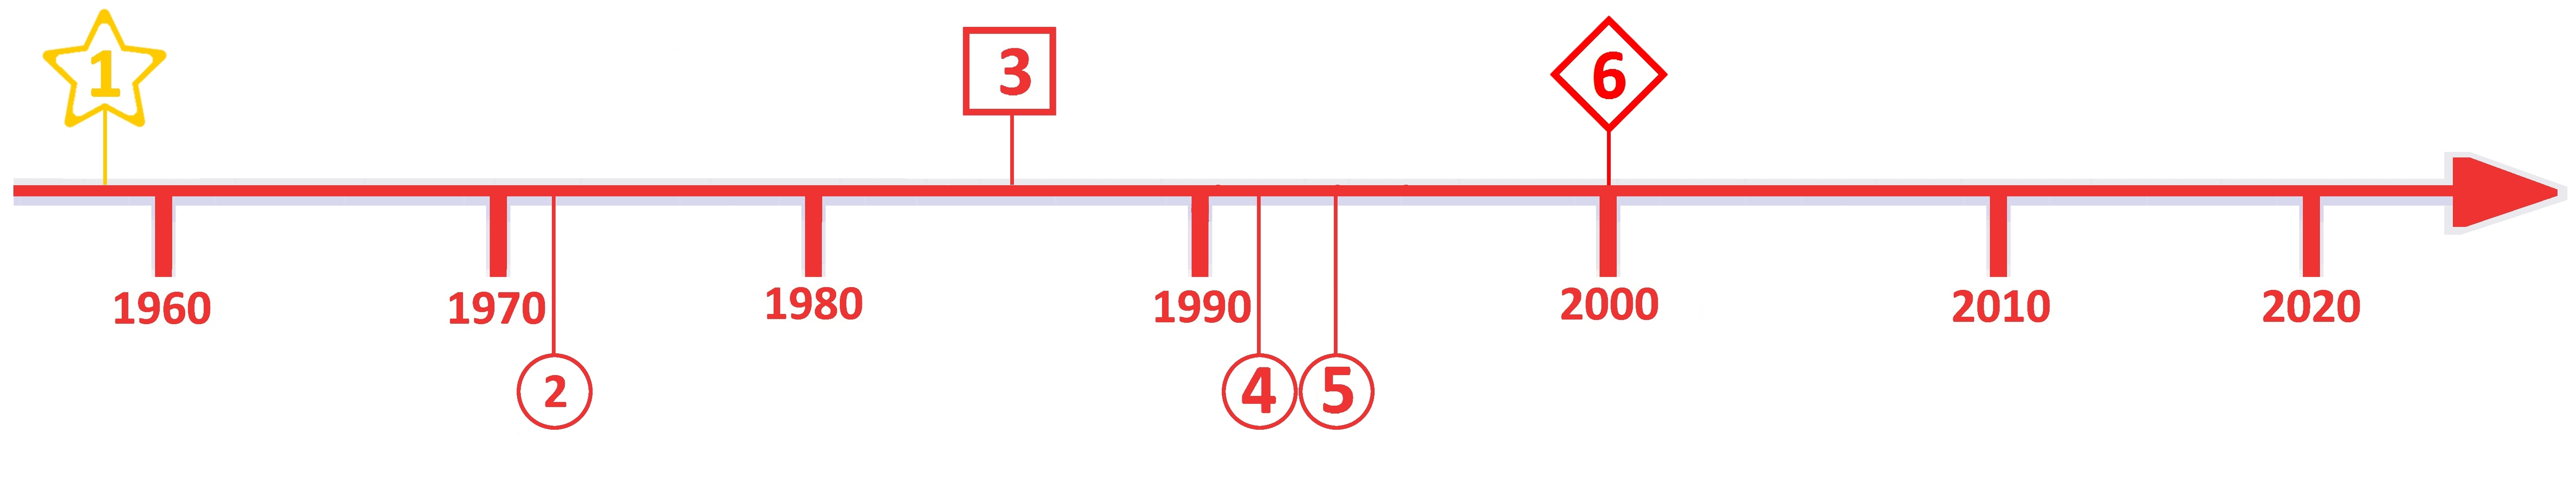
\includegraphics[width=\textwidth]{Kapitel/C-Netz/Grafiken/Zeitstrahl}
\par
\noindent
\rowcolors{2}{}{\topicolor!20}
\begin{tabular}{p{0.5 cm}p{1.5 cm}p{15.55 cm}}
	Nr. & Datum & Entwicklungsschritte~\cite{c-netz.7}\\
	1 & 1958 & Inbetriebnahme des A-Netzes: bis 1977 durch die \textit{Bundespost} (woraus unter Anderem die \textit{Deutsche Telekom} hervorging).\\
	2 & 1972 & Inbetriebnahme des B-Netzes bis 1994. \\
	3 & 1985 & \textit{DeTeMobil} stellt offiziell das C-Netz zur Verfügung.\\
	4 & 1992 & Die \textit{Deutsche Telekom} startet offiziell das D-Netz.\\
	5 & 1993 & \textit{E-Plus} startet das E-Netz.\\
	6 & 2000 & Einstellung des C-Netzes am 31.12.2000.
\end{tabular}
\par
\begin{multicols}{3}

\begin{Figure}
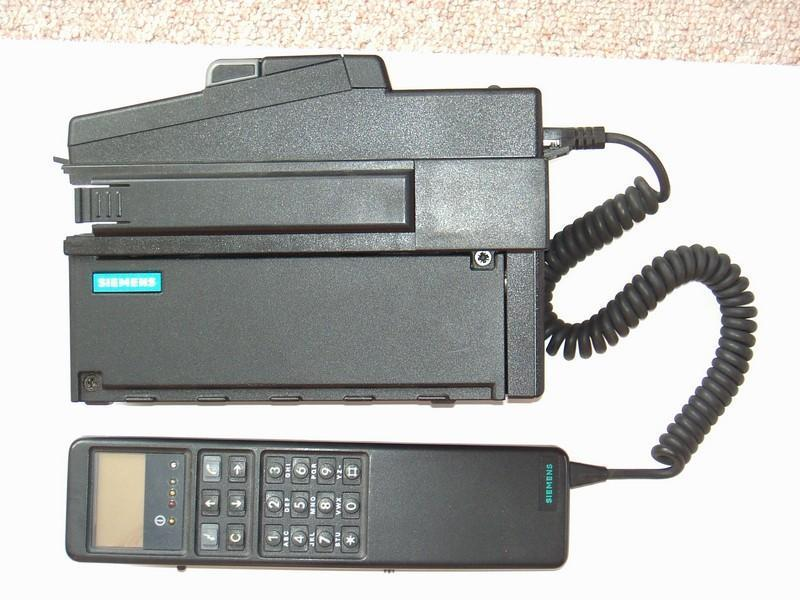
\includegraphics[width=\linewidth]{Kapitel/C-Netz/Grafiken/SiemensC1.jpg}
\captionof{figure}{Mobiltelefon~\cite{c-netz.8}}
\label{fig:c-netz.mobiltelefonZwei}
\end{Figure}
Auch auf Seeschiffen in Küstennähe Deutschlands war ein C-Netz-Gerät an Bord lange weiter verbreitet. Während der Zeit der deutschen Wiedervereinigung 1990 konnten westdeutsche Besitzer von C-Netz-Telefonen bei Aufenthalten in Ostberlin ihr Telefon benutzen und ersparten sich die zeitraubende Zuweisung eines Ferngespräches im DDR-Festnetz~\cite{c-netz.3}.
Der Betrieb des C-Netzes, das am 1. Mai 1985 startete, wurde am 31. Dezember 2000 eingestellt, mit Ausnahme einiger Funkzellen an der deutsch-niederländischen Grenze, die noch einige Monate weiterbetrieben wurden.

\subsection*{Ausblick}
Die Frequenzen des C-Netzes sollen in Zukunft für Railnet (Internet im Zug) genutzt werden. Die Telekom, die das C-Netz bis in das Jahr 2000 betrieb, ist mit ihrer Tochtergesellschaft \textit{Telekom Deutschland} bei Railnet vertreten. Für die Versorgung im Zug wird WLAN verwendet. Die Verbindung zwischen Zugserver und den stationären Antennen wird mithilfe von Flarion realisiert. Die Datenübertragungsraten von Flash-\textbf{OFDM} (\textbf{O}rthogonal \textbf{F}requency-\textbf{D}ivision \textbf{M}ultiplexing) liegen kumuliert maximal bei 3,2 Mbit/s, dabei ergeben sich für den Downlink ca. 2,5 Mbit/s und den Uplink ca. 800 kbit/s. Der große Vorteil gegenüber \textbf{UMTS} (\textbf{U}niversal \textbf{M}obile \textbf{T}elecommunications \textbf{S}ystem) sind die geringen Latenzzeiten von unter 50 Millisekunden und eine integrierte Quality-of-Service-Unterstützung. Somit steht jedem Benutzer im Zug eine Breitbandverbindung zur Verfügung. 
Die nordamerikanische Firma \textit{Flarion Technologies} ist der Entwickler der Flash-OFDM-Technik. Insgesamt sind rund 150 Stationen von Flarion bundesweit auf Sendung. Damit ist eine Abdeckung der Bahnlinien Dortmund–München und Frankfurt am Main–Hamburg gewährleistet (Stand: November 2010)~\cite{c-netz.3}.
Das praktisch unmögliche Roaming in Netze der Nachbarländer war zugleich ein Hauptgrund für die Entwicklung der nächsten Netztechnologie, die erstmals mit dem D-Netz ab 1992 zum Einsatz kam~\cite{c-netz.1}. (Bildquelle:~\cite{c-netz.9})

\printbibliography[segment=6,heading=subbibliography]
\end{multicols}
\begin{Figure}
\centering
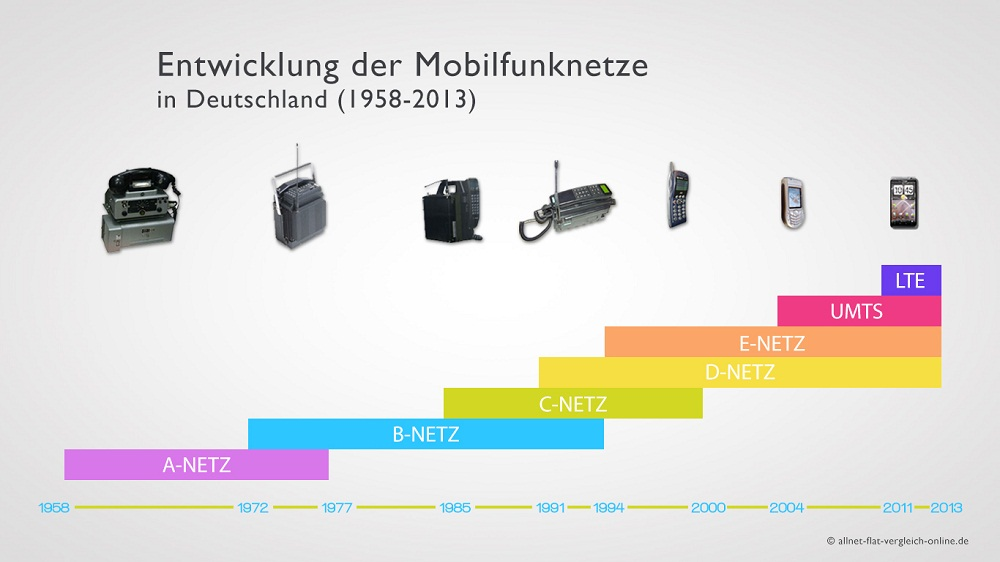
\includegraphics[height=51mm]{Kapitel/C-Netz/Grafiken/ueberblick.jpg}
\captionof{figure}{Zeitliche Übersicht von A-Netz bis LTE (Stand 2013)~\cite{c-netz.9}}
\end{Figure}

\newpage
